\subsection{Исследование свободный процессов в цепи первого порядка}

\begin{figure}[!h]
  \centering
  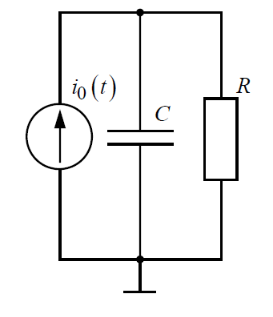
\includegraphics[width=4cm]{scheme_first_order.png}
  \caption{Схема для исследования}
  \label{fig:scheme_first_order}
\end{figure}

Соберём схему, изображённую на рис. \ref*{fig:scheme_first_order}.
Подключим к выходу генератора напряжения прямоугольной формы.
Снимем осциллограммы напряжения на конденсаторе в цепи (рис. \ref*{fig:oscillograph_first_order}).

\begin{figure}[!h]
  \centering
  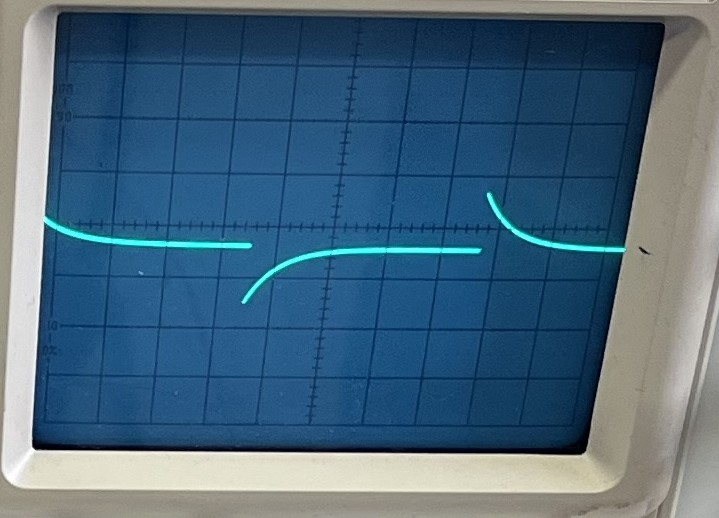
\includegraphics[width=0.8\textwidth]{oscillograph_first_order.JPG}
  \caption{Осциллограмма напряжения в цепи первого порядка}
  \label{fig:oscillograph_first_order}

\end{figure}

\subsubsection{Расчеты по осциллограмме}

По осциллограмме напряжения на конденсаторе получим значение постоянной времени $\tau = 0.08$ мс
(см. рис. \ref*{fig:culculations_first_order}).
Найдем собственную частоту цепи $p_1 = -\frac{1}{\tau} = -\frac{1}{0.08 \cdot 10^-3} \approx - 12$ кГц.

\begin{figure}[!h]
  \centering
  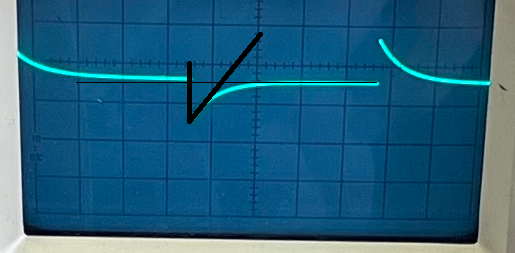
\includegraphics[width=0.6\textwidth]{ебейшие вычисления.png}
  \caption{Осциллограмма напряжения на конденсаторе}
  \label{fig:culculations_first_order}
\end{figure}

\subsubsection{Теоретические расчеты}

Найдем теоретически собственную частоту цепи:

\begin{equation}
  p_1 = -\alpha = -\frac{1}{RC}
  = -\frac{1}{5 \cdot 10^3 \cdot 0,02 \cdot 10^{-6}} \approx -10 \text{ кГц}
\end{equation}

\subsubsection{Вопросы}

1. Каким аналитическим выражением описывается
осциллографируемый процесс?

Осциллографируемый процесс описывается аналитической формулой
\begin{equation}
  u(t)
  = A e^{p_1 t}
  = A e^{-\alpha t}
  = A e^{-\frac{t}{\tau}}
\end{equation}
где u - напряжение на коком-либо элементе цепи; t - время; $\alpha$ -
постоянная затухания; $\tau$ - постоянная времени; A - постоянная интегрирования,
$p_1$ - собственная частота(вещественная и отрицательная).

2. Соответствует ли найденная собственная частота теоретическому расчету?

Найденная собственная частота цепи $p_1 = -12$ кГц, теоретическая же собственная частота цепи
$p_1 = -10$ кГц. Таким образом, найденная собственная частота цепи соответствует теоретическому расчету.

